\chapter{Introduction}
In the traditional sense, harmonic analysis relates to a set of music theory studies that pretend to describe the relationship of simultaneous sonorities and generalize rules of how each of the voices involved should move to facilitate and embellish these simultaneous sonorities.

It is difficult, however, to give a precise definition of where the task of harmonic analysis starts and finishes. As will be discussed in the literature review, different researchers have made different characterizations of the problem, sometimes binding these characterizations closely to the mathematical tools they have used to approach the problem, in other cases to the type of music that they pretend to analyze, and in other cases, it could be due to other circumstances. For this particular work, I intend to define harmonic analysis based in two simple definitions, and afterwards, the outcome definition will help to describe which are the expected inputs and outputs of an automatic harmonic analysis system.

\section{Automatic harmonic analysis}
According to the Oxford Music Online dictionary, the term analysis could be defined as the following: \cite{oxfordanalysis}

\begin{quote}
\centering
\emph{[...] the interpretation of structures in music, \linebreak
their resolution into relatively simpler constituent elements, \linebreak and the investigation of the relevant functions of those elements.}
\end{quote}

Additionally, according to the same source, a very simplistic definition of harmony could be: \cite{oxfordharmony}

\begin{quote}
\centering
\emph{The simultaneous sounding (i.e. combination) of notes [...]}
\end{quote}

Combining these definitions, one possible interpretation of what is a harmonic analysis could be the following:

\begin{quote}
\centering
\emph{[...] the interpretation of \textbf{harmonic} structures in music, \linebreak
their resolution into relatively simpler \textbf{harmonic labels}, \linebreak and the investigation of the relevant functions of those \textbf{labels}.}
\end{quote}

Therefore, as stated by this definition, the process of harmonic analysis comprises three steps:

\begin{itemize}
  \item Interpreting the harmonic structures in music
  \item Resolving these harmonic structures into harmonic labels
  \item Investigating the relevant functions among these labels
\end{itemize}

For breaking down the steps of the analysis, we could use a fragment of a musical score.

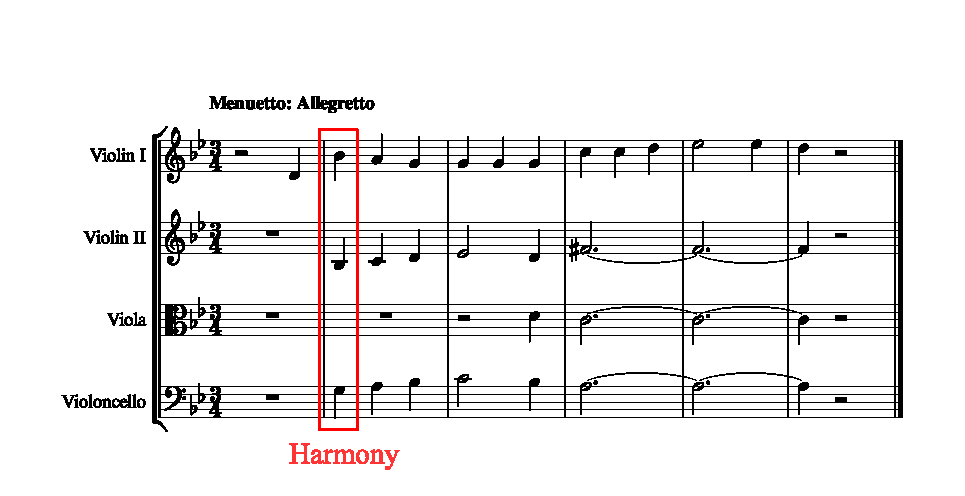
\includegraphics{figures/1}

\section{Motivation}
The main reason why it would be benefical for musicians and musicologists to automate a harmonic analysis is because it takes a considerable amount of time and knowledge to perform these analyses. In practice, students at conservatoires often learn the guidelines of harmonic analysis during a specialized course of Harmony. Such a course could extend to several years, making it a difficult discipline to learn fast for a beginner. Even in the case of experts, it might take relatively long time to analyze a piece of music in terms of harmony, which makes the task of automating it valuable even for the expert theorist.

\section{Objectives}
This work pretends to reproduce and apply the current approach for automatic functional harmonic analysis used over the KernScores corpora, and apply it to a specific set of string quartets from Joseph Haydn. Once these automatic analyses are performed, they will be compared to manual annotations over the same set of string quartets.

\section{Structure of the Report}
Literature. Methods. Results. Discussion.

\newpage
